\documentclass[12pt]{article}
\usepackage{float}
\usepackage{graphicx}
\usepackage{caption}
\usepackage{subcaption}
\usepackage{blindtext}

\title{Cellular Simulation and Population Properties}
\date{2023\\ December}
\author{Sean Donaldson\\ STAT-4000}
\begin{document}
\maketitle
\section{Abstract}

	A simulation of a colony of single-cell organisms that were capable of evolving was performed to understand the behavior of the colony.
	The analysis shows that there is a maximum of 16.9\% chance of cells undergoing several successive mutations from the binomial distribution.
	Furthermore, it can be seen that successive generations that occur from mutation have a, roughly, normal distribution for the mean of their population size.
	The mean size of a given generation has been estimated, with 95\% confidence interval, to be $CI_G = [21.75, 27.06]$ colony members.
	The total population for a given moment in time is the sum of the sub-population of all of the generations that are present for said given moment in time.
	With this in mind, observing the correlations in cell attributes for the entire population can give an idea of the overall behavior of how the colony mutates.
	It was shown that the amount of energy a cell burns per timestep, burn rate, is strongly correlated to the amount of energy a cell gains from eating food, food quality, with a value of 0.92.
	However, this correlation is the exception rather than the rule because the analysis shows that most attributes have a weak correlation with each other.



\pagebreak
\section{Introduction}

	Life as we know it has been derived from single-cell organisms. 
	Single-cell organisms can express interesting behavior in their own right. 
	However, understanding the evolution of generations of cellular organisms can provide a broader view of the behaviors of single-cell organisms.
	A custom simulation was written in C++ to try and emulate the behavior of multiple cells within a confined space.
	With this simulation, this report aims to try to statistically determine patterns and qualities of the population.
	Understanding patterns and qualities of the population of cells is key to understanding their survivability and could be a key to improving the simulation.

\section{The Simulation}

	A custom simulation engine was written to try and understand the process of evolution within a colony of cells. 
	For the simulation, it's important to understand that single-cell organisms behave independently, but are reactive to the environment around them. 
	Thus, there are many key mechanics which drive the behavior of each cell. 
	However, three major components define the simulation. 
	The three major factors which drive the simulation are the board, the cell, and the food. 
	The board is the simulation space where the cells may move around. 
	It is defined as a square matrix, $M_{n}$, where n is some integer. 
	Food is defined as some integer, $i$, which is inserted into the board matrix, and is consumed by the cell. 
	For some index on the board, $I = M_{i,j}$, the amount of food on the index can be $0 \leq I \leq 9$. 
	Food is inserted into the board matrix in two ways. 
	Prior to starting the simulation, a random amount of food is added. 
	During the simulation, a random amount of food is incrementally added to a random number of board indices every $\Delta T$ seconds where $\Delta T$ is a constant and arbitrary amount of time.

	The cells are defined both individually and as a colony. The colony is defined as a matrix $C_n$ where the maximum number of cells is $n^2$. 
	Each cell has attributes that define its needs. 
	The first attribute is Energy, $E$, which is equal to the total amount of energy the cell has for a given step in time. 
	The cell will continue to live until $E > 0$. 
	The energy a cell has may be changed by two quantities, Burn Rate, $BR$, and Food Quality, $FQ$. 
	Burn Rate is the rate that a cell's energy, $E$, drops per step in time, and Food Quality is the amount of energy a cell gains from consuming one piece of food. 
	Lastly, two attributes deal with reproduction. 
	There is a Reproduction Limit, $RL$, and Birth Penalty, $BP$. 
	The reproduction limit is defined as the minimum $E$ value the cell must have to undergo asexual reproduction, and the Birth Penalty is a number that defines how much energy the cell loses upon asexual reproduction. 
 
	How each cell moves about the board space is irrelevant to this analysis. 
	However, it will be briefly covered here. 
	If a cell is sitting on some board index, $I$, where to amount of food on the index is greater than zero then the cell will sit and consume food until the amount of food on the index reaches zero. 
	Each cell has a line of sight that is defined as a $3x3$ matrix around the cell, where the cell is at index $(2,2)$. 
	If there is food within this matrix, the cell will move to the index with the highest amount of food. 
	If there is no food within the line of sight matrix, the cell will undergo a random walk until the cell finds food, or dies from starvation, $E \leq 0$.

\section{Definitions}

	Prior to understanding the analysis, it is important to understand the defining features of the simulation.
	Except for section 7, all data shown pertains to a board size of $M_{50, 50}$. 
	furthermore, every simulation was run with 7000 timesteps where one timestep is one calculation cycle. 
	In other words, one timestep is a single cycle for all cells to complete a single action such as consuming food, moving, or reproducing.

\section{Reproduction}

	To understand the statistics of a population, it is essential to understand how the population reproduces. 
	Each cell belongs to a generation. 
	When the cell's energy is about the reproduction limit, the cell may undergo asexual reproduction. 
	Upon asexual reproduction, the child cell may undergo mutation. 
	If the child cell does undergo mutation, then the child cell will belong to a newer generation of mutated cells. 
	It's important to note that, except for the starting generation, cells in a generation do not have identical attributes.

\section{Mutations}

	Whenever a cell undergoes asexual reproduction, the child of the cell may undergo mutation. 
	Four attributes may be mutated which are Burn Rate, Food Quality, Reproduction Limit, and Birth Penalty. 
	The mutation of each child is controlled by a mutation generator. 
	The mutation generator takes some pseudo-random value $R$ where $0 \leq R \leq 25$. 
	If $R \leq 3$ then the cell undergoes mutation. Thus, the probability of mutation $P_{m} = \frac{3}{26} = 11.5\%$ for each instance of reproduction. 
	If a child cell does not undergo mutation, then the child cell will inherit the properties of its parent. 

	With a constant probability for mutation and a binary outcome, either the cell does or does not mutate. 
	The behavior of mutation can be described by a Bernoulli probability mass function where $X\sim$ Bernoulli$(\frac{3}{26})$. 
	However, with multiple cells being able to mutate and create new generations, the behavior of mutation must be with a binomial distribution.
	Thus, to determine the behavior of mutation we must define the probability mass function for mutation as $X \sim Bin(n, p)$ where n is the number of generations, 
	and p is the probability of mutation $\frac{3}{26}$. Using the data from the completed simulation, it observed that 54 generations were produced, so is set to $n = 54$.

	\begin{figure}[H]
		\caption{}
        \label{fig:}
		\centering
		\begin{subfigure}[b]{0.49\textwidth}
			\centering
			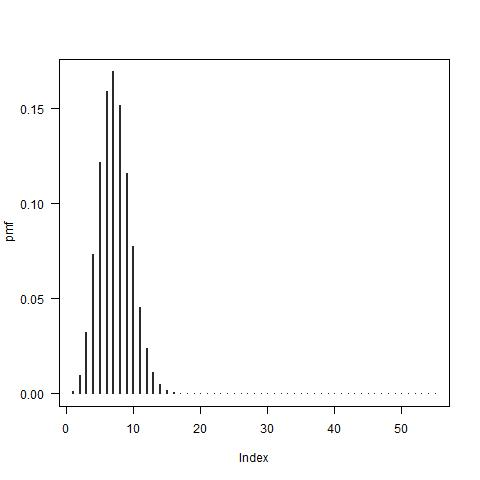
\includegraphics[width=\textwidth]{pmf.jpeg}
			\caption{$X \sim Bin(54, \frac{3}{26})$}
			\label{fig: Figure 1}
		\end{subfigure}
		\hfill
		\begin{subfigure}[b]{0.49\textwidth}
			\centering
			\label{fig: Figure 2}
			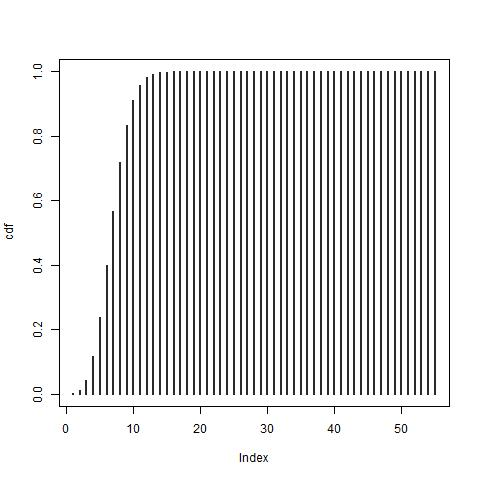
\includegraphics[width=\textwidth]{cdf.jpeg}
			\caption{$\sum_{k=1}^{54} Bin(k, \frac{3}{26})$}
		\end{subfigure}
		
   \end{figure}

	Figure 1.a shows the probability mass function for $X \sim Bin(54, \frac{3}{26})$, and figure 1.b shows the cumulative density function of the pmf. 
	We can see that for a given lineage of cells, we have a maximum of 16.9\% chance of the lineage to undergo 7 successive mutations.

  
\section{Population Means and Holding Capacity}

   Prior to understanding the behavior of the mutations within the colony of cells, it's important to understand the generations of cells that make up the population.
   For a quick look back at how the generations work, the very first cells on the board are all members of Generation 0.
   When a Generation 0 member reproduces and the child mutates, the child will be a member of Generation 1.
   This process of successive generations continues until the colony dies from starvation, or the simulation finishes.

   As a more successful generation will have more members, it is important to understand the size of each generation. 
   Figure 2, below, is a histogram showing the mean population of a generation during its lifetime, for all generations in the simulation.

	\begin{figure}[H]
		\caption{}
		\label{fig:}
		\centering
		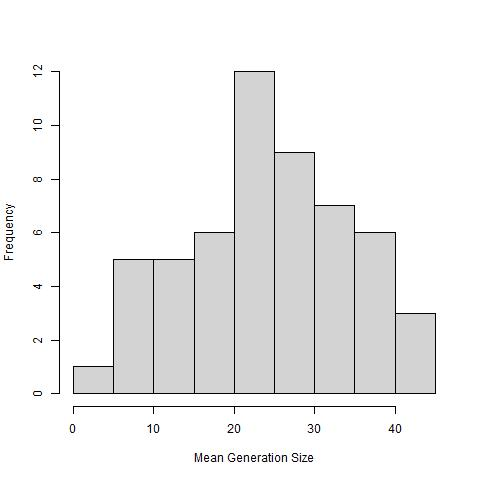
\includegraphics[width=.5\textwidth]{genHist.jpeg}
	\end{figure}
	\pagebreak
	\begin{figure}[H]
		\begin{subfigure}[b]{\textwidth}
			\center
			\textbf{Equation 1: } $CI = [\bar{x_g} - z \frac{\sigma}{\sqrt{n}}, \bar{x_g} + z \frac{\sigma}{\sqrt{n}}]$ 
		\end{subfigure}
	\end{figure}

	We can see that the population means are roughly normal. 
	With this, we may determine a confidence interval for the mean of any subsequent generation.
	Using equation 1, $z$ is set to a value of 1.96 to find a 95\% interval, $\bar{x_g}$ is the mean of all generations sizes, $\sigma$ is the standard deviation, and $n=54$ is the number of generations.

	Equation 1 shows that the mean value $\bar{x} = 24.41$, and that $CI_G = [21.75, 27.06]$. 
	For verification, a t-test was performed resulting in a mean value $\bar{x_g} = 24.41$ and $CI_G = [21.68, 27.13]$.

	Holding capacity, $HC$, can be defined as the mean of the entire population divided by the maximum number of cells. 
	Holding capacity is crucial for understanding the behavior of the population because it defines the average population size that a given board size can support.
	We can use equation one to define a confidence interval for the holding capacity of a given board. 
	However, instead of using $\bar{x_g}$, we must use $\bar{x_p}$ which is the mean population size of the entire simulation. 
	We must also define the standard deviation as the standard deviation of the population and $n$ is equal to the number of timesteps. 
	Thus, $n = 7000$.
	
	\begin{figure}[H]
		\begin{subfigure}[b]{\textwidth}
			\center
			\textbf{Equation 2: } $CI_{HC} = \frac{CI_P}{m^2}$ 
		\end{subfigure}
	\end{figure}

	To grasp the understanding of how the holding capacity affects the population, a single confidence interval is insufficient.
	Therefore, four simulations were run for $n = 7000$ where each simulation had a different board size. 
	The board sizes that were run were $10x10$, $25x25$, $40x40$, and $50x50$. 
	The confidence interval for the mean population size for each of the board sizes was determined using Equation 1.
	The maximum number of cells that can exist within the board at one time is, approximately, equal to the the board dimension squared.
	Thus, to find a confidence interval for the holding capacity, we may use equation 2 where $m$ is 10, 25, 40, and 50, and z is set to 1.96 for a 95\% confidence level.

	\begin{table}[H]
		\caption{}
		\label{fig: Table 1}
		\centering
		\def\arraystretch{1.5}%
		\scalebox{1}[1]{
		\begin{tabular}{|c|c|c|}
		\hline
			m & $CI_P$ & $\frac{CI_P}{m^2}$ \\ \hline
			10 & [62.5, 63.3] & [.625,  .633] \\ \hline
			25 & [244.1,  253.1] & [.391,  .405] \\ \hline
			40 & [396.4,  417.9] & [.248,  .261] \\ \hline
			50 & [427.3,  455.6] & [.171, .182] \\ \hline
		\end{tabular}}
	\end{table}

	Looking at these four points we can see that the holding capacity has similar behavior to $\frac{1}{x}$.
	Of course, more data points would provide a superior analysis of the behavior of the holding capacity. 
	Furthermore, using a method such as the method of least squares would be able to provide an estimated function for the behavior.
	However, such an analysis is not necessary considering the behavior of the holding capacity can be easily discerned.
	We see that as the size of the board increases, the holding capacity of the board decreases.
	Thus, we can estimate that the colony has a limited ability to propagate throughout the board.

\section{Correlations in Population}

	We now have a grasp on the understanding of the behavior of individual mutations and a confidence interval for the mean of a given generation.
	With this information, we can now look at how the population is affected by its mutations.
	Table 2 shows the correlation values between four previously mentioned values and two new ones. 
	To quickly recap, $RL$ is the reproduction limit, $FQ$ is the food quality, $BR$ is the burn rate, and $BP$ is the birth penalty.
	The two new variables are population, $P$, and food total, $FT$, for a given timestep.
	$P$ was chosen, rather than generation size for two reasons. 
	First, with 54 generations the entire population was chosen for simplicity. 
	Second, observing how mutations affect the population as a whole provides a deeper understanding rather than the relatively short lifespan of a single generation.
	
\begin{table}[H]
	\caption{}
	\label{fig: Table 2}
    \centering
    \begin{tabular}{|c|c|c|c|c|c|c|}
    \hline
        ~ & RL & FQ & BR & BP & P & FT \\ \hline
        RL & 1.00 & -0.23 & -0.24 & -0.40 & -0.11 & -0.18 \\ \hline
        FQ & -0.23 & 1.00 & -0.21 & 0.92 & 0.28 & -0.34 \\ \hline
        BR & -0.24 & -0.21 & 1.00 & -0.10 & -0.06 & 0.60 \\ \hline
        BP & -0.40 & 0.92 & -0.10 & 1.00 & 0.29 & -0.23 \\ \hline
        P & -0.11 & 0.28 & -0.06 & 0.29 & 1.00 & -0.15 \\ \hline
        FT & -0.18 & -0.34 & 0.60 & -0.23 & -0.15 & 1.00 \\ \hline
    \end{tabular}
\end{table}

	Looking at the correlation values we can see some interesting behavior. 
	We can see that most values are mildly correlated to one another, and some are weakly related to another.
	However, we can see that food quality and birth penalty are strongly correlated with a value of 0.92.
	Thus, as the food quality increases then the birth penalty also increases, and vice versa.
	We can also see that the food total and burn rate are well correlated with a value of 0.60.
	Thus, as the amount of food available to the cells increases so too does their burn rate.

\section{Discussion}

	From the analysis, we can see that the majority of mutations that occur are highly likely to have successive mutations from parent to child.
	It could be assumed that mutations that survive throughout the simulations would most likely be ones that increase the survivability of the colony.
	However, the analysis shows a much different story.
	Not only does the colony have a limited capacity for growth, shown by the holding capacity, but the mutations that persist could be hurting the colony's survivability.
	To explain further, the positive correlation value for food total, $FT$, and burn rate, $BR$, shows an inherent weakness in the colony.
	As the supply of food available to the colony increases, the weaker members of the colony are allowed to survive and pass on their attributes to their children.
	The ability of weaker cells to survive and reproduce other, potentially weaker, cells which in turn weakens the entire colony as the number of weak cells increases.

	To improve the simulation, finer control of the mutations may be needed. 
	A better method of mutation could be to give each mutatable attribute its own possibility of mutation rather than having all attributes mutate at once.
	However, to improve the growing capacity of the colony, further analysis of the holding capacity is needed.
	In order to improve the holding capacity of the colony, stronger correlation values are needed throughout the entire spectrum of variables.

\end{document}